\section{Code Base piattaforma robotica}
I punti fondamentali di una codebase per la gestione di una piattaforma robotica sono:
\begin{itemize}
    \item \textit{Digital-twin}. Questo elemento è essenziale per sfruttare librerie di pianificazione della traiettoria come MoveIt. Il modello simulato della piattaforma, che include il robot e l'ambiente di lavoro, consente a tali librerie di pianificare traiettorie che considerano la reale configurazione spaziale del manipolatore. Questo, combinato con i piani di sicurezza definiti tramite l'interfaccia proprietaria di Universal Robots, garantisce un utilizzo sicuro del manipolatore.
    \item \textit{Software di controllo del sistema multi-camera}, necessario per la gestione delle 4 telecamere che caratterizzano il complesso manipolatore-banco da lavoro.
    \item \textit{Software di teleoperazione}, necessario per il collezionamento delle traiettorie da utilizzare come esempi nel paradigma del Learning from Demonstration o del Offline Reinforcement Learning.
    \item \textit{Interfaccia per il controllo del manipolatore tramite controllori AI-based}, necessario per l'effettivo controllo del robot tramite l'utilizzo dei sistemi di AI ottenuti a valle degli addestramenti tramite imitation o rinfornzo.
\end{itemize}

\noindent Per quanto riguarda lo stato realizzativo dei punti sopra citati si possono definire tutti completati, con le relative componenti softare utilizzabili per attività di collezionamento del dataset e controllo del robot.

\section{Protocollo di Acquisizione Dataset}
Al fine di avere un protocollo di generazione degli esempi caratterizzato da elevata ripetibilità  e elevata copertura dello spazio delle azioni del robot si è deciso di definire una serie di regole che determinano il posizionamento degli oggetti da manipolare sul piano di lavoro durante la generazione degli esempi.
Come esempio verrà considerato il task di Pick and Place, ma gli stessi concetti sono possono essere generalizzati ad altri task come il Nut-Assembly.
\subsection{Pick-Place}
\begin{figure}[h]
    \centering
    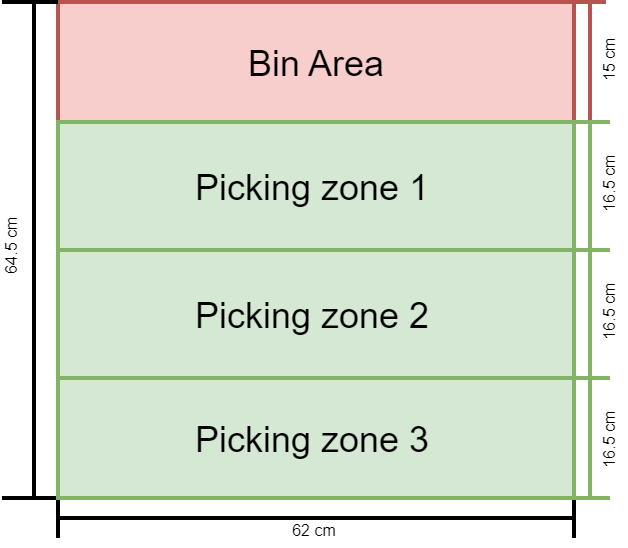
\includegraphics{Figure/Image/Dataset.png}
    \caption{Suddivisione degli spazi del workspace}
    \label{fig:workspace}
\end{figure}
In Figura \ref{fig:workspace} è possibile osservare come a partire dal tavolo di dimensioni $100\times100 \ cm$ è stato definito un workspace effettivo di $64.5 \times 62 \ cm$, diviso in 4 zone. La prima zona di ampiezza pari a $15 \ cm$ dedicata al posizionamento dei bin, mentre le restanti 3 zone di ugual ampiezza, sono dedicate per il posizionamento degli oggetti da prelevare, oggetti che in questo caso coinvolgono 4 box.
\begin{figure}[h]
    \centering
    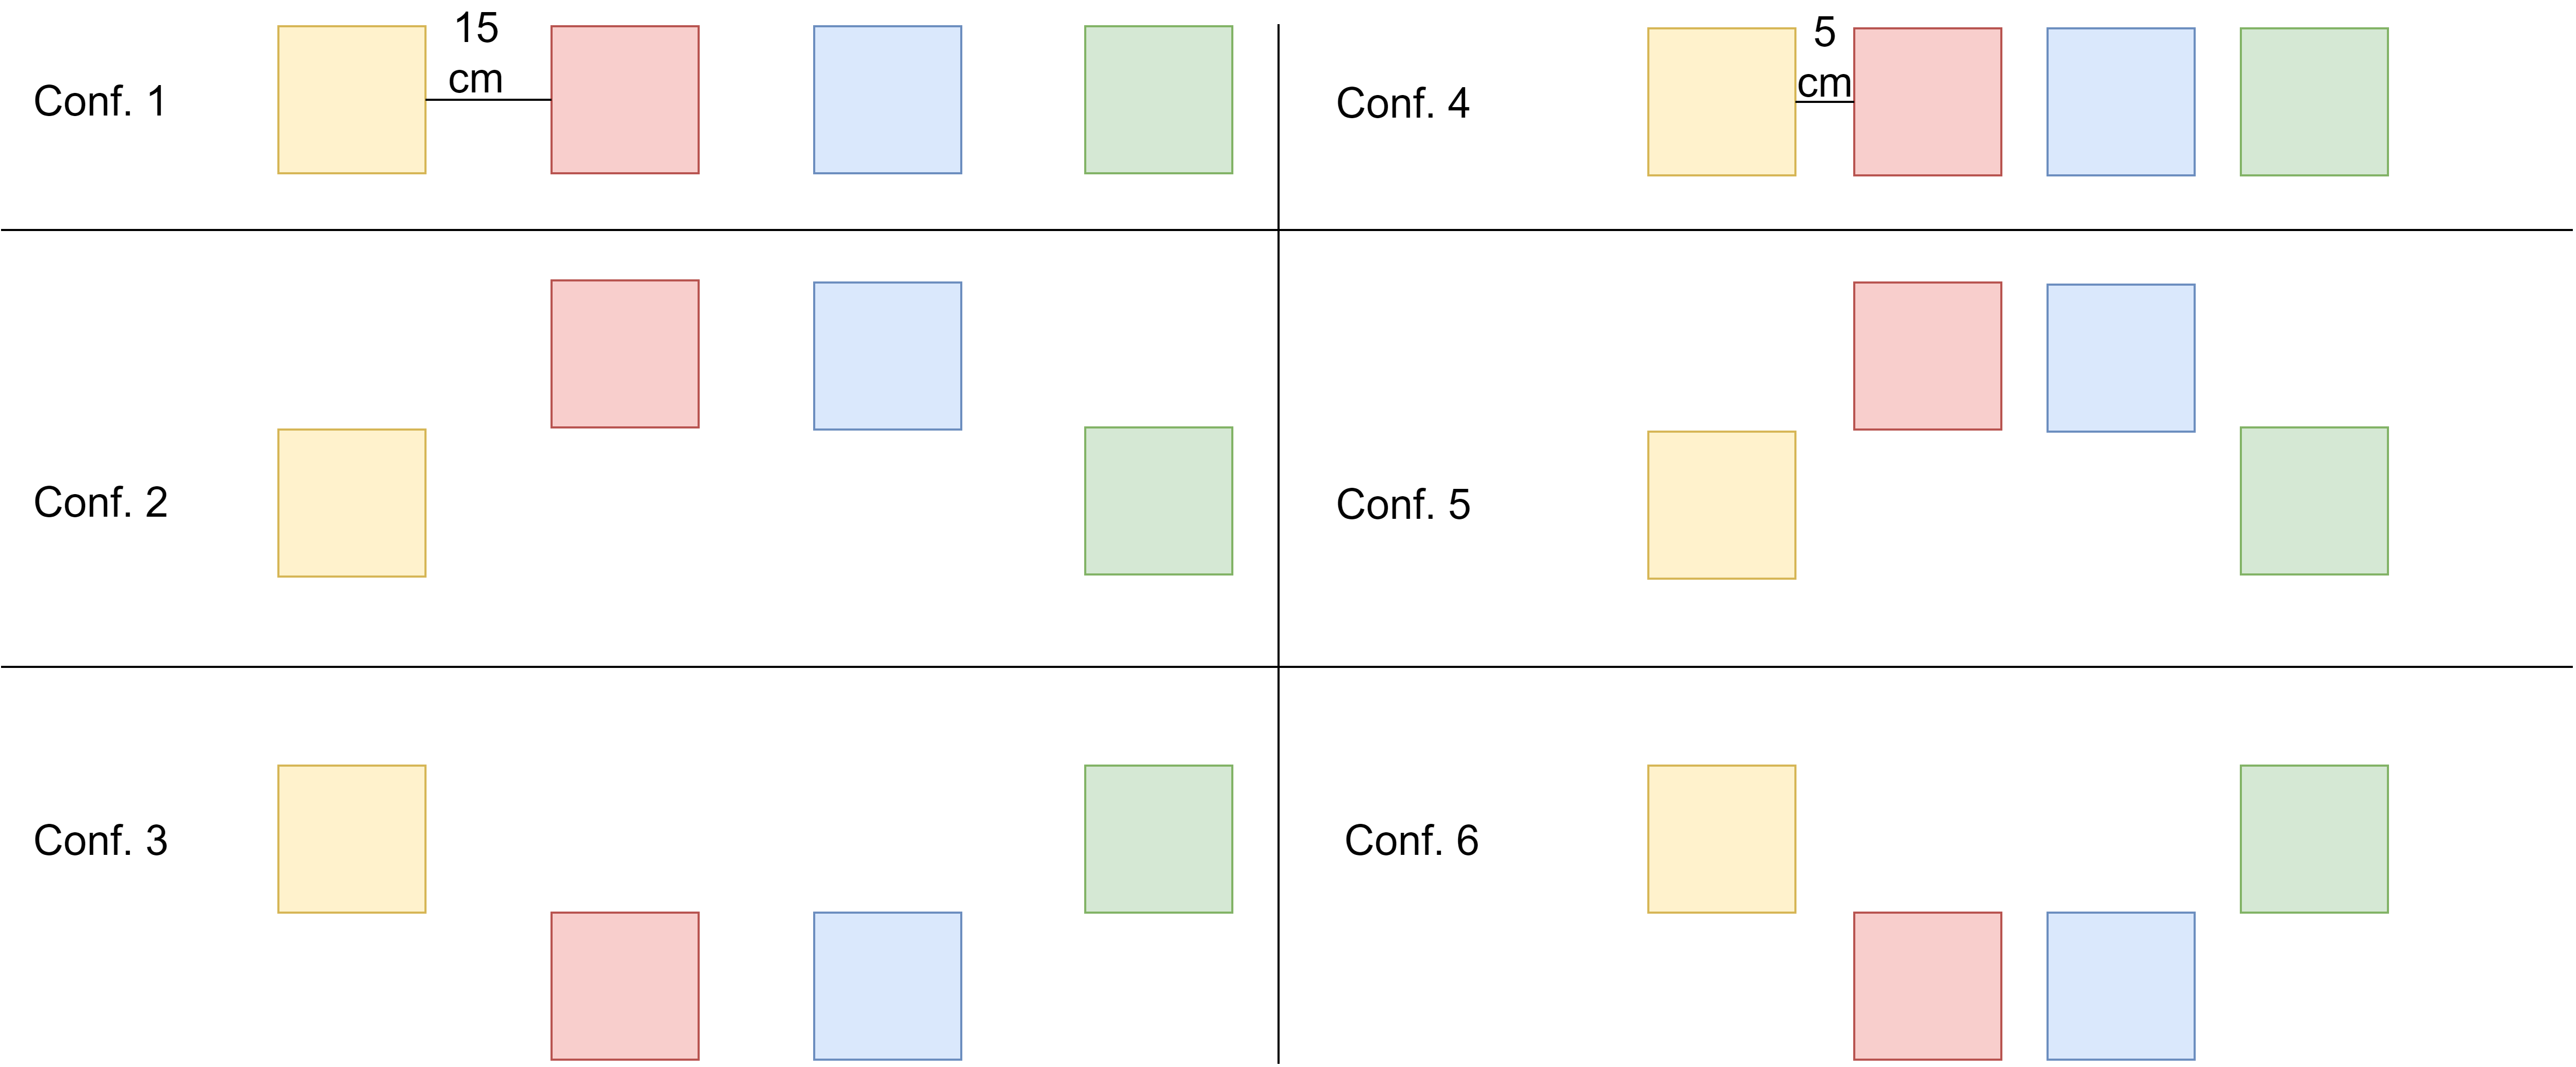
\includegraphics[scale=0.5]{Figure/Image/configurazioni.png}
    \caption{Configurazioni oggetti}
    \label{fig:configurazioni}
\end{figure}
Sono stati quindi individuate 6 possibili configurazioni di posizionamento dei box da utilizzare in ogni \textit{Picking zone}. Le configurazioni sono riportate in Figura \ref{fig:configurazioni}.
\newline Per ogni configurazione l'oggetto target andrà a coprire ogni possibile slot, andando quindi a generare 4 traiettorie per ogni configurazione.
In totale, fissato il task (e.g. Pick blocco verde e place nel primo bin) si genereranno $3 \times 6 \times 4 = 72$ traiettorie.
\newline Sulla base degli esperimenti fatti per completare il dataset per un task saranno necessarie al massimo $ 4 hrs$. Questo tempo è stato abbondantemente sovrastimato per la gestione di eventuali errori e riesecuzione di traiettorie.
Quindi per il completamento del dataset di \textit{Pick and Place} che include 16 task saranno necessarie $64 \ hrs$.
Al momento secondo questo protocollo sono stati collezionati 1 task su 16.

\section{Training Framework}
Per quanto riguarda la codebase legata al Framework di addestramento questa si può ritenere \textbf{utilizzabile}. Dato che la procedura di addestramento non cambia tra il dataset simulato e il dataset reale.